\documentclass{article}

% *** CITATION PACKAGES *** 

\usepackage{cite}

% *** GRAPHICS RELATED PACKAGES *** 

\usepackage[pdftex]{graphicx}
\usepackage{tikz}

% *** MATH PACKAGES ***

\usepackage{amsmath} 
\usepackage{amssymb} 
\usepackage{amsthm}
\usepackage{latexsym} 
\usepackage{amstext}
\usepackage{amsxtra} 
\usepackage{amsfonts} 
\usepackage{graphicx}


\usepackage{algorithmic}
\usepackage{algorithm}

% *** ALIGNMENT PACKAGES *** 


\usepackage{array} 
\usepackage{mdwmath}
\usepackage{mdwtab} 

\usepackage[tight,footnotesize,caption=false]{subfig}

% *** CITATION PACKAGE *** %
% ** IJRR asks for an author-date bibtex style ** %
\usepackage{harvard}


\newtheorem{theorem}{Theorem}


\begin{document}
\title{Dynamic Walking makes Humanoid Robot Small-Space Controllable: Application to Motion Planning}

\author{
S\'ebastien Dalibard\and
Antonio El Khoury\and
Florent Lamiraux\and
Michel Ta\"ix\and
Jean-Paul Laumond
\footnote{The authors are with CNRS ; LAAS ; 7 avenue du colonel Roche, F-31077
  Toulouse Cedex 4, France and Universit\'e de Toulouse ; UPS, INSA, INP, ISAE ; UT1, UTM, LAAS ; F-31077 Toulouse
  Cedex 4, France.}
\footnote{A preliminary version of this paper appeared in the 11th 
  IEEE-RAS International Conference on Humanoid Robots, 2011.}
}

 


\maketitle


\begin{abstract}
  This paper presents humanoid robot  \textit{small-space controllability}: 
  a theoretical result with practical
  consequences on dynamic walk motion planning.
  Based on it, we propose 
  a  two-stage motion planner for walking humanoid
  robots.  A first draft path is computed using probabilistically complete
  random motion planning  techniques that  ensure collision avoidance.  
  In a  second step, the
  draft path  is approximated by a whole-body  dynamically stable walk
  trajectory.   The  contributions  of  this  work are:  (i)  a  formal
  guarantee,  based on small-space  controllability criteria,  that the
  first draft path can be approximated by a collision-free dynamically
  stable  trajectory; (ii)  an  algorithm that  uses this  theoretical
  property to find  a solution trajectory. We have  applied our method
  on several  problems where whole-body planning and  walk are needed,
  and the results have been validated  on a real  platform: the robot
  HRP-2.
\end{abstract}


\section{Introduction}

Since early results on planning for car-like robots \cite{taix-94}, it has been known that 
controllability properties can be used to simplify planning algorithms. In particular,
small-time controllability accounts for the fact that from any given starting point,
the reachable space in limited time $t$ of a system always contains a neighborhood 
of this point. This property has a very specific implication in motion planning:
any collision free path can be approximated  by  a sequence  of  both  
collision-free and  admissible trajectories. 

This leads to a two-step well grounded planning approach for small-time 
controllable systems:
\begin{enumerate}
\item Plan a collision-free path using any geometric planning algorithm
\item Apply an approximation scheme on this path, using the controllability property
\end{enumerate}
On the other hand, when planning for walking systems, dynamic stability 
is often seen as a constraint accounting for a growth of algorithmic 
complexity. Indeed, trying to consider both a system geometric state and its 
dynamics at the  planning phase results in a combinatorial explosion of
the size of the spaces to explore. When planning whole-body trajectories for humanoid
robots, as opposed to 2D navigation planning, this growth of complexity
is not compatible with close to real-time applications.


In this work, we prove that walking humanoid robots are small-space 
controllable, a property similar to small-time controllability.
Applying this result, we propose a two-step planner for 
whole-body collision-free trajectories that require stepping.
\begin{itemize}
\item In  a first stage, a randomized motion
  planner computes a collision-free, statically stable path for a humanoid 
  robot whose feet
  are sliding  on the  ground. At this stage, only geometric constraints are considered.
\item In  a second stage,  this draft  path is
  approximated by  a dynamically stable walk  trajectory. 
\end{itemize}
We  present 
various examples of use  of this algorithm in
the  experimental section  of the  paper.  The  experiments  have been
conducted  on a  model of  the HRP-2  robot, and  validated on  a real
platform, see Fig. \ref{fig:couv}.


\begin{figure}[h]
\centering
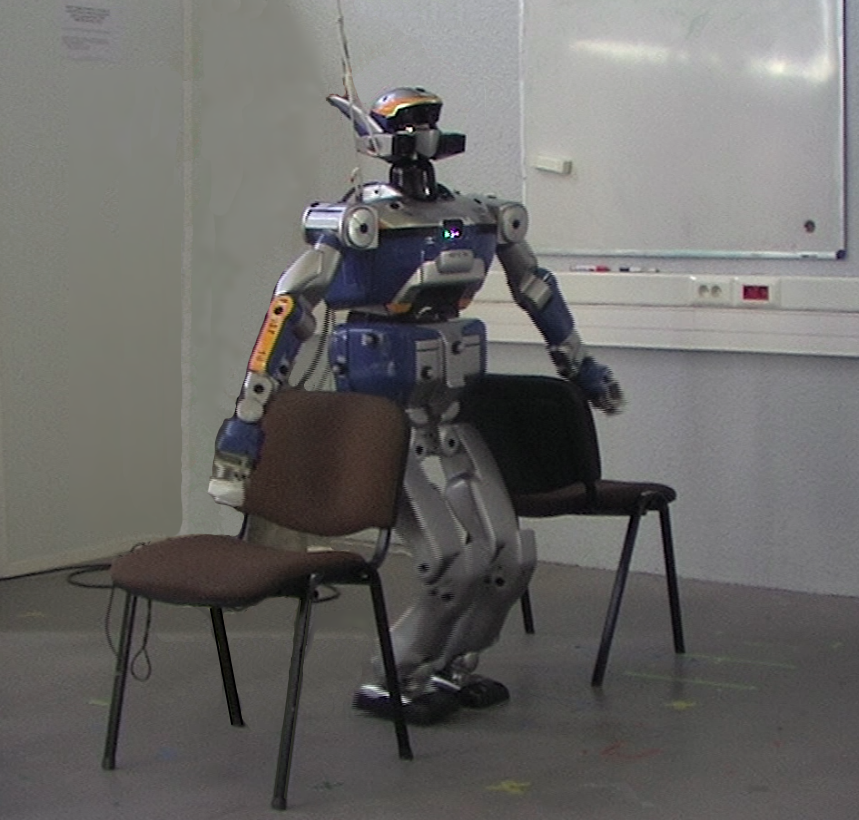
\includegraphics[width=0.6\linewidth]{pics/chairs/couv.png}
\caption{The robot HRP-2 passing between two chairs. In this kind of
  environment whole-body collision avoidance is needed during
  locomotion.} 
\label{fig:couv}
\end{figure}


\subsection{Outline}

Section \ref{sec:related-work} summarizes the related work found in the literature;
section \ref{sec:sliding} describes the first step of our approach: geometric
motion planning; section \ref{sec:ssc}
introduces the concept of \textit{small-space controllability} and applies it to humanoid robots;
section \ref{sec:animation} describes the global planning algorithm proposed in this paper; 
and finally section \ref{sec:exp} shows some applications of the method.


\section{Related Work and Contribution}
\label{sec:related-work}

This work is based on two different fields of humanoid robotics
research:  first  randomized  whole-body  motion
planners and second walk pattern generators based on the Zero-Momentum
Point (ZMP) formalism.  These two fields  rely at a lower level on the
prioritized inverse kinematics (IK)  formalism
\cite{siciliano1991gfm,nakamura1986iks}. 
Collision-avoidance
can be integrated into an IK-solver, \cite{kanehiro2008lca} presents such a method for
whole-body motion planning, and \cite{OussamaKanoun06102010} for collision avoidance at a
footstep placement level. However, these methods are prone to fall
into local minima. In this paper, we focus on global motion
planning. 


\subsection{Whole-Body Motion Planning}

When  planning a  whole-body motion  for a  humanoid robot,  the first
challenge is to cope with  the curse of dimensionality. The complexity
of   motion  planning  is   exponential  in   the  dimension   of  the
configuration  space ($\mathcal{CS}$)  to explore.  When  dealing with
high-dimensional configuration  spaces, it is  typically impossible to
explicitly represent  them, leading to the use  of randomized sampling
techniques  to solve  global planning  problems. In  the  past fifteen
years,  \textit{Probabilistic Roadmaps} \cite{kavraki1996prp} and  
\textit{Rapidly exploring Random  Trees} (RRT) 
\cite{kuffner00rrtconnect}  have been  developed and  used to  solve many
high dimensional   planning  problems.
When  using  sampling  techniques  on  a humanoid  robot,  the  second
difficulty  is to  take into  account stability  constraints,  i.e. to
generate  random  configurations   on  zero  volume  submanifolds  of
$\mathcal{CS}$. This problem has been investigated with success during
the last few years, \cite{Berenson15032011,dalibard09} present some 
solutions. The idea is to use
prioritized  inverse  kinematics techniques  within  the framework  of
sampling-based motion planning. To our knowledge, recent contributions
to this field do not cover walk planning.

\subsection{Walk pattern generation}

Another  field of  humanoid  robotics research  is  the generation  of
dynamically stable  walk patterns. Since  the introduction of  the ZMP
formalism  \cite{vukobratovic1969contribution},  several  methods  have  been  proposed  to
generate  walking  motions efficiently.   One  way  to  deal with  the
complexity  of a  humanoid  robotics  kinematic tree  is  to use  the
so-called "cart-table" simplified model \cite{kajita2003biped}. Based on such a
model,  planning a trajectory  for the  ZMP is  reduced to  planning a
trajectory  for  the Center  of  Mass (CoM)  of  the  robot.  Given  a
trajectory  of  the CoM  and  footstep  positions, inverse  kinematics
solvers can animate  the whole set of degrees of freemdom (DoFs) of the  
robot to generate a dynamically stable walk trajectory.

\subsection{Collision-free Walk Trajectories}

Collision-free  locomotion   trajectories  are  usually   obtained  by
simplifying the model of the  robot or of its environment. By choosing
a bounding volume of a  humanoid robot, including its swaying motions,
one can  use a simple  planar motion planner  on this bounding  volume and
generate  a valid  locomotion  trajectory. This  strategy  is used  in
\cite{pettre20032} in a computer animation context. Variants of this method
include  dynamic path reshaping  \cite{yoshida-humanoids05}: if  collisions appear
when animating  the locomotion  trajectory, it is  locally reshaped
and re-animated.  This two-stage  strategy does not guarantee that the
locomotion trajectory can be followed or that the local reshaping will
converge.

Simplifying  the environment  consists in  considering obstacles  at a
footstep   level.   \cite{chestnutt2005footstep,kuffner2005motion}
use   an  
A$^{*}$   algorithm  to   find
collision-free   footsteps.    In   \cite{perrinbiped},   the   authors   compute
collision-free motions  for the legs by using  an RRT$^{*}$ algorithm. 

Some planning methods for free-climbing robots \cite{bretl2006motion}
can be seen as a general way 
to consider quasi-static multi-step planning, they are not directly applicable to
humanoid dynamically stable locomotion.
Other recent contributions to the field of locomotion planning  include algorithms 
considering the dynamics at the planning phase \cite{shkolnik2011bounding}. This leads to 
a growth of algorithmic complexity, particularly costly for high-dimensional
systems such as humanoid robots. In our work, we show that it is not always
necessary to take into account dynamics while planning, even though the final
output of our algorithm is a dynamically stable walk motion.

\subsection{Contribution}

The main contribution of this work is a two-stage motion planner for a
humanoid robot that computes a collision-free walking trajectory on the
exact models of the robot and its environment. The first stage uses a
sampling-based motion 
planner to  compute a collision-free path  for a robot  sliding on the
ground. Another  contribution of this  paper is the formal  proof that
this path can be  approximated by a dynamically stable, collision-free
walking  trajectory. We have implemented this method and  used it on a
model of  HRP-2 robot.  The results have been  validated on a real
platform.



\section{Statically stable collision-free path for a "sliding" robot}

\label{sec:sliding}

The first stage  of our planning architecture consists  in computing a
statically stable  path for  a humanoid robot  sliding on  the ground.
The static  stability of the configurations of the
robot along this path is defined by the following constraints:
\begin{enumerate}
\item The two  feet are on the ground, and  their relative position is
  fixed,
\item The robot CoM is projected vertically in  the center of its
  support polygon. 
\end{enumerate}
To ensure that the sliding path  can be approximated by a dynamically
stable  trajectory,  we add the constraints used to validate 
the cart-table model approximation:
\begin{enumerate}
\setcounter{enumi}{2}
\item The robot CoM is at a constant height,
\item The robot waist is kept vertical.
\end{enumerate}

Random  motion planning  under task  constraints has  been successfully
investigated in the past years. Here, we apply the method described in
\cite{dalibard09}. Note  that all the constraints  applied on the  robot at that
stage are  expressed in the  robot frame, so the  non-articular DoFs
describing the global  position and orientation of the  robot are free
to change.

\begin{figure}
\centering

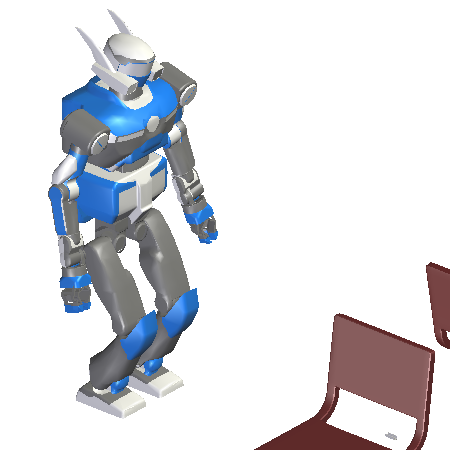
\includegraphics[width=0.24\linewidth]{pics/chairs/sliding-perspective-1.png}
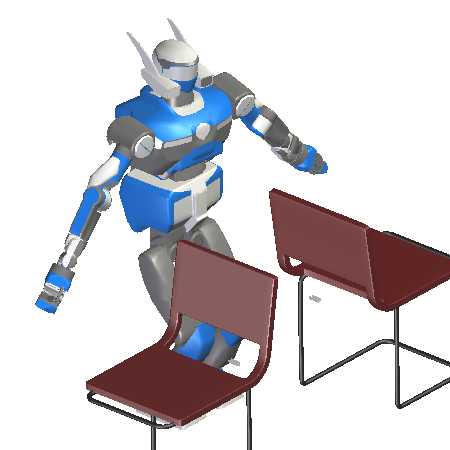
\includegraphics[width=0.24\linewidth]{pics/chairs/sliding-perspective-2.png}
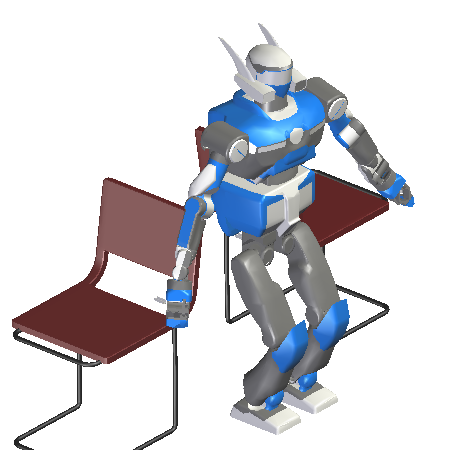
\includegraphics[width=0.24\linewidth]{pics/chairs/sliding-perspective-3.png}
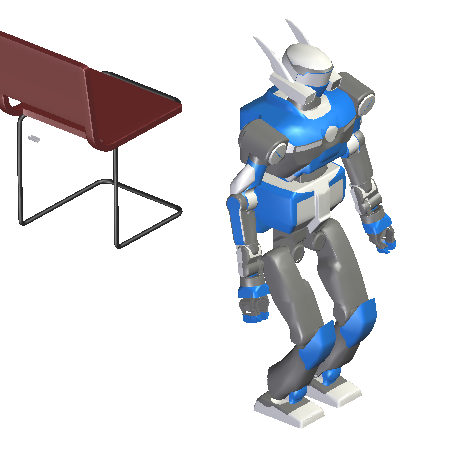
\includegraphics[width=0.24\linewidth]{pics/chairs/sliding-perspective-4.png}



\caption{Collision-free  statically stable path  for a  humanoid  robot  sliding on  the
  ground.}
\label{fig:sliding}
\end{figure}


Fig. \ref{fig:sliding} shows an example of a collision-free path found
by an RRT algorithm. All the configurations along the path respect the
set of constraints listed above. The CoM height and the feet positions
in the robot frame are chosen such that the generated 
configurations avoid singularities.


\section{Existence of a dynamically stable trajectory}

\label{sec:ssc}

This  section presents a proof that  any sliding path
$p$  can be approximated  by a  collision-free walk  trajectory.  This
property is based on ideas from control theory, and in
particular small-space  controllability. Let  us recall briefly  what a
small-space controllable  system is, and  how this property is  used in
motion planning.

\subsection{Small-Space Controllability}

A  robotic system  is  controllable  if  for any two  configurations
$q_1$ and $q_2$,  there exists  a  time  $T>0$ such  that  there exists  a
trajectory  going  from  $q_1$ to  $q_2$  in  time  $T$.  It  is  
small-time  controllable if for  any configuration  $q$, for  any time
$T>0$, the set of configurations accessible from $q$ in time less than
$T$ is a  neighborhood of $q$ in $\mathcal{CS}$.  In geometric terms,
and if velocities and accelerations are bounded, the following formulation is
equivalent:
for any  configuration $q$, for any $\epsilon >0$, there
exist $\eta >0$ such that all the configurations contained in the ball of center
$q$ and radius $\eta$ are reachable by trajectories included in the
ball of center $q$ and radius $\epsilon$.
We will refer to this geometric 
formulation as {\it small-space controllability}. 

The main  consequence of  the small-space controllability property  
in  motion planning  is that  any
collision-free path (not necessarily  admissible by the system) can be
approximated  by  a sequence  of  both  collision-free and  admissible
trajectories.  It is  crucial  in  nonholonomic  motion  planning
\cite{laumond1998robot}. Fig. \ref{fig:stc} shows an example of collision-free 
path approximation by admissible collision-free sub-trajectories. The fact 
that this algorithm  converges is guaranteed by the small-space
controllability property.

\begin{figure}
  \centering

  \begin{minipage}{3cm}
    
\definecolor{cc6c6c6}{RGB}{198,198,198}
\definecolor{cffffff}{RGB}{255,255,255}

\begin{tikzpicture}[y=0.4pt, x=0.4pt,yscale=-1, inner sep=0pt, outer sep=0pt]
% path5273
\path[shift={(-0.42857142,4.7142857)},draw=black,miter limit=4.00,line
  width=0.800pt]
  (365.7143,269.5050)arc(0:180:97)arc(-180:0:97) --
  cycle;

% path5275
\path[shift={(-6.0609153,-3.535534)},draw=black,fill=cc6c6c6,miter
  limit=4.00,line width=0.800pt]
  (323.7539,278.0803)arc(-0:180:51)arc(-180:0:51) --
  cycle;

% path5315
\path[draw=black,line join=miter,line cap=butt,miter limit=4.00,line
  width=1.200pt] (265.6701,275.0498) .. controls (265.6701,275.0498) and
  (165.7228,265.2948) .. (178.2919,306.8696) .. controls (185.4208,330.4496) and
  (285.8732,311.9204) .. (285.8732,311.9204) -- (285.8732,311.9204);

% path4761
\path[draw=black,fill=cffffff,miter limit=4.00,line width=0.400pt]
  (278.8021,274.5447)arc(0:180:12)arc(-180:0:12) --
  cycle;

% path4761-4
\path[shift={(17.677674,33.840124)},draw=black,fill=black,miter limit=4.00,line
  width=0.400pt]
  (278.8021,274.5447)arc(-0:180:12)arc(-180:0:12) --
  cycle;

% text5307
\path[fill=black] (288,334.92981) node[right] (text5307) {$q'$};

% text5311
\path[fill=black] (280,286.9537) node[above right] (text5311) {$q$};

% path5319
\path[draw=black,fill=black,line join=miter,line cap=butt,line width=0.800pt]
  (201.0204,312.4254) -- (220.7183,318.9914) -- (200.5153,323.0320) --
  (201.0204,312.4254) -- cycle;

% path2829
\path[draw=black,line join=miter,line cap=butt,line width=0.800pt,<->]
  (273.5714,264.5050) -- (320.0,191.6479);

% path2831
\path[draw=black,line join=miter,line cap=butt,line width=0.800pt,<->]
  (254.2857,270.2193) -- (226.4286,245.2193);

% text2833
\path[fill=black] (302.14285,231.6479) node[above right] (text2833) {$\epsilon$};

% text2837
\path[fill=black] (242.14285,258.07648) node[above right] (text2837) {$\eta$};


\end{tikzpicture}

  \end{minipage}
  \begin{minipage}{4cm}
    
\definecolor{cd9d9d9}{RGB}{217,217,217}
\definecolor{c888888}{RGB}{136,136,136}
\definecolor{cc8c8c8}{RGB}{200,200,200}

\begin{tikzpicture}[y=0.65pt, x=0.65pt,yscale=-1, inner sep=0pt, outer sep=0pt]
  \begin{scope}% layer1
    % path4348-7-9
    \path[cm={{0.88069687,0.0,0.0,0.88069687,(30.925926,8.8427197)}},draw=black,fill=cd9d9d9,miter
      limit=4.00,fill opacity=0.450,line width=0.273pt]
    (347.2399,152.3163)arc(0:180:14)arc(-180:0:14) --
    cycle;

    % path4348-7-9-7
    \path[cm={{1.1259005,0.0,0.0,1.1259005,(-41.191,-23.012876)}},draw=black,fill=cd9d9d9,miter
      limit=4.00,fill opacity=0.450,line width=0.213pt]
    (347.2399,152.3163)arc(0:180:14)arc(-180:0:14) --
    cycle;

    % path5244
    \path[draw=c888888,dash pattern=on 1.60pt off 3.20pt,line join=miter,line
      cap=butt,miter limit=4.00,line width=0.800pt] (324.7640,142.9724) .. controls
    (324.7640,142.9724) and (392.3443,194.3298) .. (397.6213,198.4045) .. controls
    (402.3196,202.0323) and (410.6305,205.8633) .. (413.9100,204.5917) .. controls
    (416.8177,203.4642) and (420.7090,195.9224) .. (421.4862,193.4800) .. controls
    (422.4768,190.3665) and (423.7590,185.6513) .. (423.7590,185.6513);

    % path2160
    \path[cm={{0.51754158,0.59470899,-0.78330399,0.64302546,(277.06748,-164.97712)}},draw=black,line
      join=miter,line cap=butt,line width=0.800pt]
    (502.2720,157.7193)arc(0:180:122 and
    86)arc(-180:0:122 and 86) -- cycle;

    % path3136
    \path[draw=black,fill=cc8c8c8,line join=miter,line cap=butt,even odd rule,line
      width=0.800pt] (323.5714,118.0765) .. controls (342.3822,104.3382) and
    (350.5113,93.1397) .. (367.8571,95.2193) .. controls (385.2029,97.2990) and
    (419.0623,103.2255) .. (417.1429,135.2193) .. controls (415.2234,167.2132) and
    (419.3643,167.7282) .. (415.3825,190.6736) .. controls (411.4008,213.6191) and
    (384.7193,178.1899) .. (372.1429,156.6479) .. controls (359.5665,135.1059) and
    (371.4345,121.3381) .. (351.4286,123.0765) .. controls (331.4227,124.8148) and
    (304.7606,131.8148) .. (323.5714,118.0765) -- cycle;

    % path3138
    \path[draw=black,fill=cc8c8c8,line join=miter,line cap=butt,even odd rule,line
      width=0.800pt] (282.8571,157.3622) .. controls (286.1376,149.2915) and
    (279.6176,144.7773) .. (334.2857,171.6479) .. controls (388.9538,198.5185) and
    (362.8864,196.4968) .. (370.7143,213.7908) .. controls (378.5422,231.0847) and
    (409.6606,211.9285) .. (414.2857,213.0765) .. controls (418.9109,214.2244) and
    (419.9284,228.7908) .. (388.5714,227.3622) .. controls (357.2145,225.9336) and
    (259.4398,220.6704) .. (282.8571,204.5050) .. controls (306.2745,188.3397) and
    (279.5767,165.4328) .. (282.8571,157.3622) -- cycle;

    % path3146
    \path[cm={{0.4204395,0.0,0.0,0.4204395,(301.97396,131.87051)}},draw=black,fill=black]
    (293.9544,127.3150)arc(-0:180:4 and
    4.798)arc(-180:0:4 and 4.798) -- cycle;

    % path3144-4
    \path[cm={{0.4204395,0.0,0.0,0.4204395,(203.23155,89.696643)}},draw=black,fill=black]
    (293.9544,127.3150)arc(-0:180:4 and
    4.798)arc(-180:0:4 and 4.798) -- cycle;

    % path4348-7
    \path[cm={{1.066689,0.0,0.0,1.066689,(-30.387755,-19.628005)}},draw=black,miter
      limit=4.00,line width=0.225pt]
    (347.2399,152.3163)arc(0:180:14)arc(-180:0:14) --
    cycle;

    % path3144-4-0
    \path[cm={{0.4204395,0.0,0.0,0.4204395,(212.23282,96.333932)}},draw=black,fill=black]
    (293.9544,127.3150)arc(-0:180:4 and
    4.798)arc(-180:0:4 and 4.798) -- cycle;

    % path4462
    \path[draw=black,line join=miter,line cap=butt,line width=0.800pt]
    (325.0000,143.5229) .. controls (325.0000,143.5229) and (337.3919,129.0073) ..
    (335.5357,136.6479) .. controls (333.5526,144.8109) and (334.2857,150.1300) ..
    (334.2857,150.1300);

    % path4348-7-7
    \path[cm={{1.3636764,0.0,0.0,1.3636764,(-119.57563,-59.410424)}},draw=black,miter
      limit=4.00,line width=0.293pt]
    (347.2399,152.3163)arc(0:180:14)arc(-180:0:14) --
    cycle;

    % path3144-4-0-5
    \path[cm={{0.4204395,0.0,0.0,0.4204395,(223.84497,105.10147)}},draw=black,fill=black]
    (293.9544,127.3150)arc(-0:180:4 and
    4.798)arc(-180:0:4 and 4.798) -- cycle;

    % path4511
    \path[draw=black,line join=miter,line cap=butt,line width=0.800pt]
    (333.9817,149.9171) .. controls (333.9817,149.9171) and (321.6451,171.4668) ..
    (337.5172,166.2059) .. controls (344.1210,164.0170) and (345.7247,159.3873) ..
    (345.7247,159.3873) -- (345.7247,159.3873);

    % path4513
    \path[draw=black,line join=miter,line cap=butt,line width=0.800pt]
    (345.7143,158.4336) .. controls (345.7143,158.4336) and (359.6429,157.0050) ..
    (363.0357,162.8979) .. controls (368.5714,168.4336) and (355.4744,164.7300) ..
    (362.0816,172.0514);

    % path3144-4-0-5-7
    \path[cm={{0.4204395,0.0,0.0,0.4204395,(240.22838,117.85464)}},draw=black,fill=black]
    (293.9544,127.3150)arc(-0:180:4 and
    4.798)arc(-180:0:4 and 4.798) -- cycle;

    % text3039
    \path[fill=black] (420.71426,173.43362) node[right] (text3039) {$q_2$};

    % text3043
    \path[fill=black] (290,141.29077) node[above right] (text3043) {$q_1$};

    % text3142
    \path[fill=black] (410.71429,90) node[right] (text3142) {$\mathcal{CS}$};

    \node (obst) at  (325,200) {Obstacles};

  \end{scope}

\end{tikzpicture}

  \end{minipage}
  
  \caption{Small-space controllability in motion planning. On the left,
    the local property: any configuration $q'$ at distance less than
    $\eta$ is reachable from $q$ by an admissible trajectory included in
    a ball of size $\epsilon$. On the right, a collision-free path from
    $q_1$ to $q_2$ is approximated by collision-free and admissible
    trajectories by using the local property.
  }
  \label{fig:stc}
\end{figure}


\subsection{Small-Space Controllability of a Walking Humanoid Robot}

We want to prove that any collision-free sliding path found by  the 
method presented
in section \ref{sec:sliding}
-~for example the one presented in 
fig. \ref{fig:sliding}~- 
can be followed by a sequence of collision-free 
walk motions. 
Let $\mathcal{M}$ be the $\mathcal{CS}$ 
submanifold formed by configurations verifying the constraints (1) to 
(4) presented in section \ref{sec:sliding}. It is then sufficient to
prove the following result:
\begin{theorem}
$\forall q \in \mathcal{M}$, $\forall \epsilon >0$,
$\exists \eta >0$ such that $\forall q' \in \mathcal{M}$ such
that $d(q,q') < \eta$, there exists a dynamically stable walk motion
going from $q$ to $q'$
included in the $\mathcal{CS}$-ball of center $q$ and radius $\epsilon$. 
\end{theorem}


The result is valid under
the hypothesis of the cart-table simplified model. We will thus 
consider that the arms are of negligible mass and do not influence the 
position of the CoM of the robot. The DoFs of the robot upper-body
are therefore free to follow exactly any input trajectory. On the other 
hand, the DoFs defining the position and orientation of the whole robot in 
space and the articular DoFs of the legs must generate a valid walk motion
and cannot follow any path. The proof will consider first the non-articular 
DoFs defining the position and orientation of the robot and then the
leg DoFs.  To position the robot in space, we will consider the
position of its CoM. 


Following the cart-table model, we require that
during the walk motion the CoM stays at a constant height and that the
global rotations of the robot around $(x)$ and $(y)$ axes are constant of
null angle, so overall, there are three non-articular DoFs of the
robot that change along a walk trajectory: $x$, $y$ and $\theta$,
where $x$ and $y$ define its CoM horizontal position, and $\theta$ the
angle of the rotation of the robot around the $(z)$ axis. 


\subsubsection{Walking in place}
\label{sec:com-stc} 

It is sufficient to show that it  is possible to walk in place while keeping
the  CoM of  the  robot  in an  arbitrarily  small neighborhood.  The
equations  giving  the   ZMP  horizontal  coordinates  $(p_x,p_y)$  as
functions  of CoM  coordinates $(x,y)$  in the  cart-table  model were
presented in \cite{kajita2003biped}:
\begin{equation}
\label{eq:walk-zmp}
\left(
\begin{array}{c}
p_x\\ p_y
\end{array}
\right) = \displaystyle \left(
\begin{array}{c}
x - \frac{z_c}{g} \ddot{x}\\ y - \frac{z_c}{g} \ddot{y}
\end{array}
\right)
\end{equation}
where $z_c$ is  the constant height of the CoM and  $g$ is the gravity
constant.    In    the    following    we    will    note    $\omega_0
=\sqrt{\frac{g}{z_c}}$.

To be able to  lift a foot without falling, the robot  has to move its
ZMP under its other foot. Let  us consider a robot in configuration
$(0,0,0)$. To move the ZMP  under a
given foot, only  the $y$ coordinate of the CoM  is of interest. Thus,
we will keep the $x$ coordinates  of the CoM and ZMP constant equal to
$0$.

We wish to walk in place while keeping the CoM in an arbitrarily small
neighborhood. Let $\epsilon >0$, arbitrarily chosen, be the size of
that neighborhood. We 
require that for  any time $t\geq 0$, $|y(t)|  \leq \epsilon$. Let $L$
be the horizontal distance between the CoM and the center of either of
the robot feet. We aim at
making $p_y(t)$ oscillate  between $-L$ and $L$. During  this proof we
will  assume that the  feet of  the robot  are rectangular,  of length
$l_1$ and width  $l_2$. If the feet are not  rectangular, we can adapt
the proof by  considering a rectangle included in  the contact surface
between  a foot  and  the ground.  If  no such  rectangle exists,  for
example if the contact is punctual, this proof does not hold.

The idea of this proof is to use the form of Eq. (\ref{eq:walk-zmp}) to
apply a  scaling factor between  the amplitude of the  oscillations of
the CoM and of the ZMP. For example for $\omega >0$, let us assume the
trajectory of the CoM is given by $y(t) = \epsilon \sin(\omega t)$. We
can derive Eq. (\ref{eq:walk-zmp}) and obtain $p_y(t) =
(1+\left(\frac{\omega}{\omega_0}\right)^2)\epsilon\sin(\omega t)$. The
amplitude  of  the oscillations  of  $y$  is  multiplied by  a  factor
$(1+\left(\frac{\omega}{\omega_0}\right)^2)$.  If we choose  $\omega =
\omega_0 \sqrt{\frac{L}{\epsilon} -1}$,  $p_y$ oscillates between $-L$
and    $L$.   At    time   $t_l^{(n)}    =    n\frac{2\pi}{\omega}   +
\frac{\pi/2}{\omega}$, the  ZMP is located  at the center of  the left
foot,  the robot  can lift  its right  foot and  at time  $t_r^{(n)} =
n\frac{2\pi}{\omega}  + \frac{3\pi/2}{\omega}$ the  ZMP is  located at
the center of the right foot, the robot can lift its left foot.


Starting from a static configuration at time $(t=0)$, we cannot apply
directly  a  command  $y(t)  =  \epsilon \sin(\omega  t)$  because  it
generates  a discontinuity  in the  speed of  the CoM  at time $(t=0)$. To
overcome this  discontinuity, we go through a  transient state between
$(t=0)$ and  $(t=T)$ for some  $T >0$. Let  $f:[0,T] \rightarrow
[0,1]$  be an  increasing function of class $C^\infty$  such  that  $f(0)  =  0$,
$\dot{f}(0) = 0$, $f(T) =  1$, $\dot{f}(T) = 0$ and $\ddot{f}(T)
=  0$.  We can explicitly  construct  such  an $f$   with  a degree  4
spline.   We   also   request   that   for  all   $t   \in   [0,T]$,
$|2\epsilon\dot{f}(t)\frac{\omega}{\omega_0^2}|   \leq  \frac{l_2}{4}$
and   $|\epsilon\ddot{f}(t)/\omega_0^2|  \leq   \frac{l_2}{4}$.  These
inequalities  will be  used  to bound  the  trajectory of  the  ZMP. We  can
guarantee them by  choosing $T$ large enough. Let  us now consider the
following CoM motion:

\[
y(t) = \left\{
\begin{array}{ll}
f(t)\epsilon\sin(\omega t) 
& \text{if } t\in [0,T]
\\ 
\epsilon\sin(\omega t) 
& \text{if } t \geq T \end{array}
\right.
\]

One can  check that $y$  is of class $C^2$ over  $\mathbb{R}_+$, and
that $\dot{f}(0) = 0$. When $t\geq T$, the robot is in the permanent
state described above  and can walk in place. The  last point to check
is that for $t \in  [0,T]$ $p_y(t)$ stays inside the support polygon
of the robot. The calculation of the successive derivatives of $y$ gives:

\[
\begin{array}{cl}
p_y(t) = &  f(t) \epsilon (1 + \left(\frac{\omega}{\omega_0}\right)^2)
\sin (\omega  t) \\ &  + 2\epsilon \dot{f}(t)\frac{\omega}{\omega_0^2}
\cos  (\omega t)  \\ &  +  \frac{\epsilon}{\omega_0^2}\ddot{f}(t) \sin
(\omega t)
\end{array}
\]


\begin{figure}
\centering
\begin{tikzpicture}[domain=0:12,x=0.07\linewidth,y=1.7cm]
  


  \draw [->] (0,-1.1) -- (12,-1.1)  ;
  \draw [->] (0,-1.1) -- (0,1.2) ;

  \node [left] (l1) at (0,-1) {$-L$};
  \node [left] (l2) at (0,1)  {$L$};
  \node [left] (0) at (0,0) {$0$};
  \node [below right] (t) at (12,-1.1) {time};
  \node [left] (e1) at (0,0.2) {$\epsilon$};
  \node [left] (e2) at (0,-0.2) {$-\epsilon$};

  \draw [thin, color=lightgray] (0,-1) -- (12,-1);
  \draw [thin, color=lightgray] (0,1) -- (12,1);
  \draw [thin, color=lightgray] (0,-0.2) -- (12,-0.2);
  \draw [thin, color=lightgray] (0,0.2) -- (12,0.2);
  

  \node [below] (0t) at (0,-1.1) {$0$};
  \node [below] (t1) at (5,-1.1) {$T_1$};

  \draw plot[only marks, mark=+] coordinates {(0,0) (0,-0.2) (0,0.2)
    (0,-1) (0,1) (5,-1.1)};

  \node [above left] at (0,1.1) {$y$};

  \node [right,color=red] at (11,0) {CoM};
  \node [right,color=blue] at (11,0.8) {ZMP};
  
  
  \draw [domain=0:5,thick,smooth,samples=100,color=red] plot[id=1] 
  function{0.2*(0.0048*x**4 - 0.064*x**3+0.24*x**2)*sin(6*x)};

  \draw [domain=5:11,thick,smooth,samples=100,color=red] plot[id=2]
  function{0.2* sin(6*x)};

  \draw [domain=0:5,thick,dashed, smooth,samples=100,color=blue] plot[id=3]
  function{
    (0.92*(0.0048*x**4 - 0.064*x**3 +0.24*x**2))*sin(6.*x)
    -(0.02*(0.0576*x**2-0.384*x+.48))*sin(6.*x)-(0.24*(0.0192*x**3-.192*x**2+.48*x))*cos(6.*x)
};

  \draw[domain=5:11,thick,dashed, smooth,samples=100,color=blue]  plot[id=4]
  function{sin(6*x)};



\end{tikzpicture}


\caption{CoM motion (in plain red) along $y$ axis.  The CoM stays in the interval
  $[-\epsilon,\epsilon]$ while during  permanent state ($t \geq T$),
  the ZMP (dashed blue) oscillates between the centers of the feet, which allows
  in-place walk.}
\label{fig:zmp-inplace}
\end{figure}

For    all     $t    \in    [0,T]$,    $f(t)     \epsilon    (1    +
\frac{\omega}{\omega_0}^2)  \sin  (\omega t)$  lies  between $-L$  and
$L$. The bounds on the derivatives of $f$ guarantee that $p_y(t)$ lies
between  $-L- l_2/2$ and  $L+ l_2/2$,  which means  that the  ZMP stays
inside  the  support  polygon.  Fig.  \ref{fig:zmp-inplace}  shows  an
example  of CoM  motion  on the  $y$  axis and  the corresponding  ZMP
motion. Once in permanent walk in-place state, the robot can come back
to  a static  state by  applying a  symmetric transient  state  used to
decrease  gradually  the amplitude  of  the  oscillations  of the  CoM
without  generating a  discontinuity in  the first  derivative  of the
command.


These CoM motions can be adapted to follow a $(x,y,\theta)$ linear
segment by a dynamically stable walk motion, while keeping the CoM at
distance at most $\epsilon$ from the segment. To do so, we add the
walk-in-place CoM motion presented above to the desired
trajectory.  The details of the proof are shown in Appendix.





\subsubsection{Legs degrees of freedom}

During a walk motion, the six  DoFs of each leg are controlled through
a position and orientation task on the foot. For a given configuration
of  the  robot  waist,  this   task  is  defined  by  six  equations
determining the position and  orientation of the foot. Let $q_{waist}$
be the configuration of the waist of the robot, $q_{foot}$ the desired
configuration of  the foot, and $q_{leg}$  the articular configuration
of  the leg.  The  task  on the  foot  is defined  by  a function  $Tk:
\mathbb{R}^6  \times   \mathbb{R}^6  \times  \mathbb{R}^6  \rightarrow
\mathbb{R}^6$,  such  that the  task  is  satisfied iff  $Tk(q_{waist},
q_{foot},  q_{leg})  =  0$.  Each   component  of  $Tk$  is  a  sum  of
trigonometric functions and  as such, $Tk$ is of  class $C^\infty$. Let
$q^{(0)}  \in  \mathcal{M}$.  By  hypothesis,  when the  robot  is  in
$q^{(0)}$,  the tasks defining  the positions  and orientation  of the
feet are  not in  singularity. Hence, $\partial  Tk /  \partial q_{leg}
(q_{waist}^{(0)},  q_{foot}^{(0)}, q_{leg}^{(0)})$ is  invertible. The
implicit  function theorem  can be  applied and  states  that: there
exist   open  sets   $U  \subset   \mathbb{R}^{12}$  and   $V  \subset
\mathbb{R}^6$ and $\phi : U \rightarrow V$ such that:
\begin{itemize}
\item  $(q_{waist}^{(0)}, q_{foot}^{(0)}) \in U$ and $
  q_{leg}^{(0)} \in V$,
\item $\forall (q_{waist}, q_{foot}) \in U, Tk(q_{waist}, q_{foot},\phi(q_{waist}, q_{foot})) =0$,
\item $\phi$ is of class $C^\infty$.
\end{itemize}

The continuity of $\phi$ implies that for any given $\epsilon$,  
there exists a neighborhood $U'\subset U$ of $(q_{waist}^{(0)}, q_{foot}^{(0)})$ such that 
footsteps corresponding to configurations in $U'$ generate leg configurations at distance 
less than $\epsilon$ from $ q_{leg}^{(0)}$.



\subsubsection{Global Proof}

We can now conclude the proof. Let $q^{(0)}$ be a configuration in
$\mathcal{M}$ and $\epsilon >0$ arbitrarily chosen. Let $U'_l$ and $U'_r$ be
open balls of $\mathbb{R}^6$ as defined above respectively for the left and right
foot. Let $V$  be the set of configurations $q \in \mathcal{M}$ such that: 
\begin{itemize}
\item the non-articular DoF values are in $U'_l \cap U'_r$
\item the non-articular DoF values are at distance at most 
	$\epsilon$ from $q^{(0)}$,
\item the upper-body DoF values of $q$ are at distance 
	at most $\epsilon$ from  $q^{(0)}$,
\end{itemize}
$V$ contains a neighborhood of $q^{(0)}$ in $\mathcal{M}$. For any $q \in V$,
the CoM and leg motions corresponding to a walk motion from $q^{(0)}$ to $q$ as described
in appendix, with a linear interpolation of the upper-body DoFs, generate a whole-body
motion at distance at most $k.\epsilon$ from $q^{(0)}$ 
where $k$ is a constant depending on the number
of DoFs of the robot. This concludes the proof. 

\subsubsection{Remarks}
\paragraph{Use of ZMP preview controller:} The control strategy presented in this proof may
generate very  long trajectories, because  of the transient  states at
the beginning and end of the locomotion. In the actual implementation,
we chose  to generate  CoM motions with  a ZMP preview  controller, as
presented in \cite{kajita2003biped}.  We  have observed experimentally that the
amplitude of  CoM trajectories decreases  when the frequency  of steps
increases.

\paragraph{Speed of CoM:} The theoretical result presented in this section implies
that any collision-free path can be approximated by a sequence of admissible 
and collision-free trajectories. However, the theorem depends on a control law
that will generate trajectories with unbounded velocities for the CoM, when the input
path is close to obstacles. The humanoid robot
hardware may be a limitation to such trajectories. To prevent the generated CoM 
oscillations from being too fast, one has to require that the statically stable 
draft path is included
inside a $\epsilon$-radius tube of the free space, where $\epsilon$ depends on the
physical capacities of the robot.

\section{Animation of the statically stable path}

\label{sec:animation}

The  algorithm   that  animates  a  statically  stable   path  into  a
dynamically stable  walk trajectory has been inspired  by the previous
small-space controllability  proof. Given a statically  stable path $p$,
we  start  by placing  footsteps  corresponding  to  the nominal  walk
pattern  of the  robot. Given the footsteps, we  compute a ZMP trajectory, 
and a preview controller outputs  a corresponding CoM trajectory. We
use  the implementation  shown in  \cite{yoshida2006tds} to  solve a
prioritized inverse kinematics problem.  The stack of tasks applied to
the robot is - in decreasing priority order:
\begin{enumerate}

\item Position and orientation of the moving foot,

\item Horizontal position of the CoM,

\item Height of the CoM,

\item Verticality of the waist,

\item Upper-body configuration task towards corresponding
  configuration  of $p$.

\end{enumerate}

Tasks (1)  and (2) generate a  dynamically stable motion  by using the
simplified cart-table model  and the ZMP criterion. Tasks  (3) and (4)
ensure that the  resulting motion is well described  by the cart-table
model. Task (5)  is used to approximate $p$ as  well as possible given
the walk parameters.

Because it comes at the  lowest priority, task (5) is not necessarily
fulfilled in  the resulting trajectory. Hence,  collisions may appear
when animating $p$, if the resulting trajectory diverges too much from
the initial sliding  path. If so, it is  necessary to approximate more
closely $p$  by a walk  trajectory.  To do  so, we use  the small-space
controllability  property   of  the  system  shown   in  the  previous
section. The way  we use this property is  inspired by similar results
in non-holonomic mobile robot control presented in \cite{taix-94}.

If the animated  trajectory collides with the environment,  we cut the
initial  path   $p$  into  two   sub-paths,  that  we  try   to  animate
recursively. When the  paths to animate are too  short for the robot
nominal  walk parameters, we  accelerate the  steps, and  decrease the
maximum height of  the moving foot. As shown  in previous section, the
walk trajectory  corresponding to  smaller and faster  steps converges
toward the  sliding path.  Algorithm  \ref{alg:walk} shows pseudo-code
that takes  a sliding path $p$  as input and  returns a collision-free
walk trajectory.

\begin{algorithm}[h]
\caption{FindDynamicTrajectory(Path $p$)}
\label{alg:walk}
\begin{algorithmic}
\STATE $Footprints \leftarrow \text{ComputeFootprints}(p)$

\STATE $StackOfTasks$.initialize()

\STATE $StackOfTasks$.addFootprintTask($Footprints$)

\STATE $StackOfTasks$.addWaistTask()

\STATE $StackOfTasks$.addConfigurationTask($p$)

\STATE $DynamicTrajectory \leftarrow \text{Animate}(StackOfTasks)$

\IF{(CheckForCollisions($DynamicTrajectory$) = Colliding)}

\STATE $(p_1,p_2) \leftarrow \text{CutInHalf}(p)$

\STATE $DT_1 \leftarrow \text{FindDynamicTrajectory}(p_1)$

\STATE $DT_2 \leftarrow \text{FindDynamicTrajectory}(p_2)$

\RETURN $\text{Concatenate}(DT_1,DT_2)$

\ELSE

\RETURN $DynamicTrajectory$

\ENDIF
\end{algorithmic}
\end{algorithm}


\section{Experiments}

\label{sec:exp}

The motion planning algorithms presented in this paper have been implemented
using KineoWorks\texttrademark \cite{laumond2006kcs}. The planning times have been measured
on an Intel Core~2~Duo 2.13~GHz PC with 2~GB of RAM. Evaluation of the
randomized algorithm has been conducted by executing 50 trials on each
problem, we present the average results.


\subsection{Passing between two chairs}


The environment shown in Fig. \ref{fig:couv} and \ref{fig:sliding} was
presented in \cite{el2011path}. The  authors solved it by using a bounding
box method, leading the robot to walk sideways between the two chairs.
Our method generated a locomotion  trajectory in which the robot walks
forward, which could be required if the robot has to use vision during
locomotion for  example. The first planning stage  required 29.6~s
on  average.   The  animation  of   the  sliding  path   presented  in
Fig.   \ref{fig:sliding}    used   66.5~s  of  computation   time.


\begin{figure}[h!]
\centering
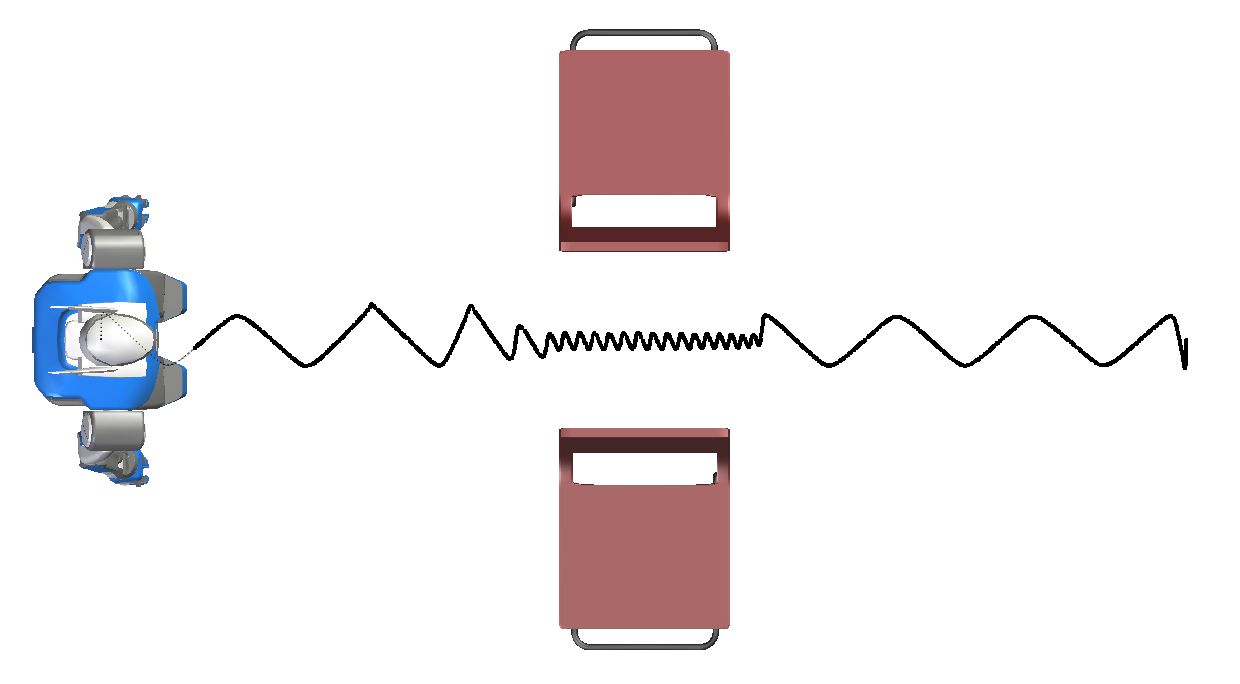
\includegraphics[width=0.7\linewidth]{pics/chairs/waist-trajectory.png}

\caption{Horizontal trajectory of the robot waist during
  locomotion. When the robot is close to obstacles, the amplitude of
  the oscillations decreases.}
\label{fig:chairs-waist}
\end{figure}



Fig.  \ref{fig:chairs-waist} shows  the horizontal  trajectory  of the
robot CoM  during  locomotion. The amplitude of the oscillations  decreases when passing
between the  chairs.  This motion has  been validated on  a real HRP-2
platform. 

\subsection{Cluttered environment}

\begin{figure}[h!]

\centering

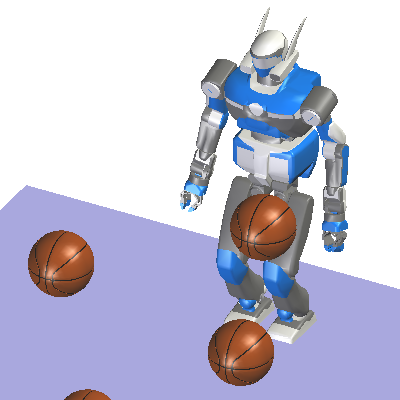
\includegraphics[width=0.24\linewidth]{pics/objects-cloud/perspective-1.png}
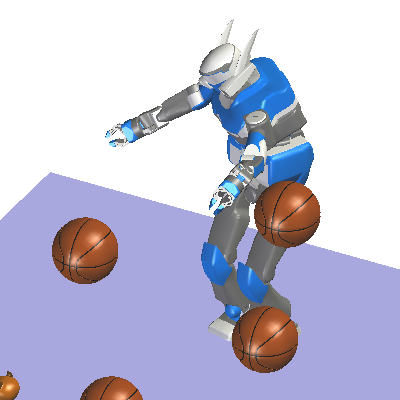
\includegraphics[width=0.24\linewidth]{pics/objects-cloud/perspective-2.png}
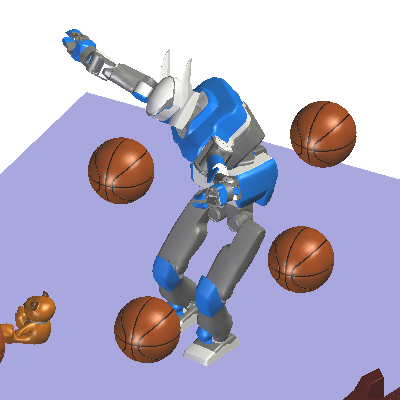
\includegraphics[width=0.24\linewidth]{pics/objects-cloud/perspective-3.png}
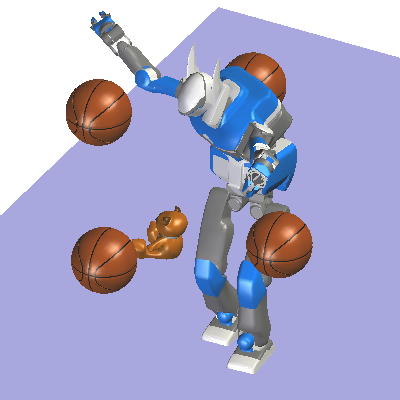
\includegraphics[width=0.24\linewidth]{pics/objects-cloud/perspective-4.png}
\\ 
\vskip 0.08cm
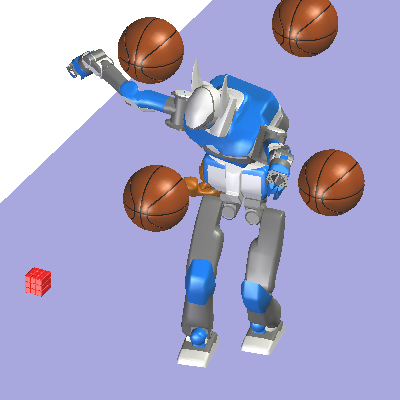
\includegraphics[width=0.24\linewidth]{pics/objects-cloud/perspective-5.png}
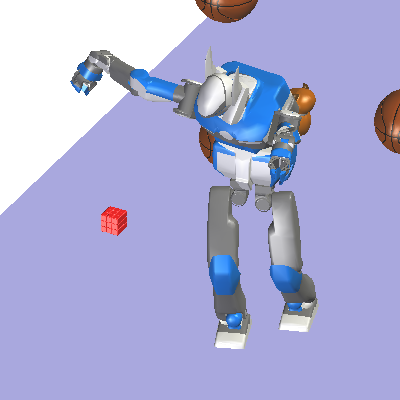
\includegraphics[width=0.24\linewidth]{pics/objects-cloud/perspective-6.png}
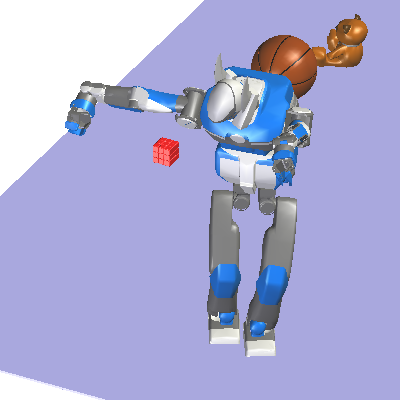
\includegraphics[width=0.24\linewidth]{pics/objects-cloud/perspective-7.png}
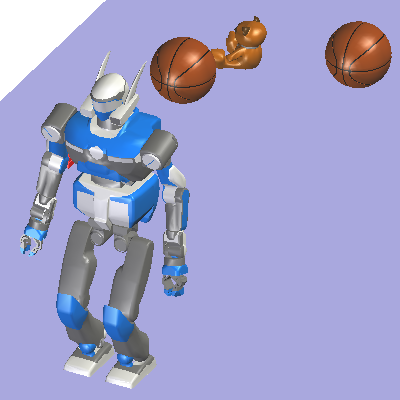
\includegraphics[width=0.24\linewidth]{pics/objects-cloud/perspective-8.png}

\caption{Solution path for a cluttered environment, the robot walks
  among floating obstacles.}
\label{fig:cluttered}
\end{figure}

In the environment shown in Fig. \ref{fig:cluttered}, the robot
has to find a way among floating obstacles. In this
environment neither bounding box nor footstep planning strategies
could find a collision-free walk trajectory.
The first planning stage required
184.3~s on average, and the animation of the trajectory presented in 
Fig. \ref{fig:cluttered} used 339.5~s of computation time. Fig. \ref{fig:cluttered-waist} 
shows the robot waist trajectory during locomotion.

\begin{figure}[h!]
  \centering
  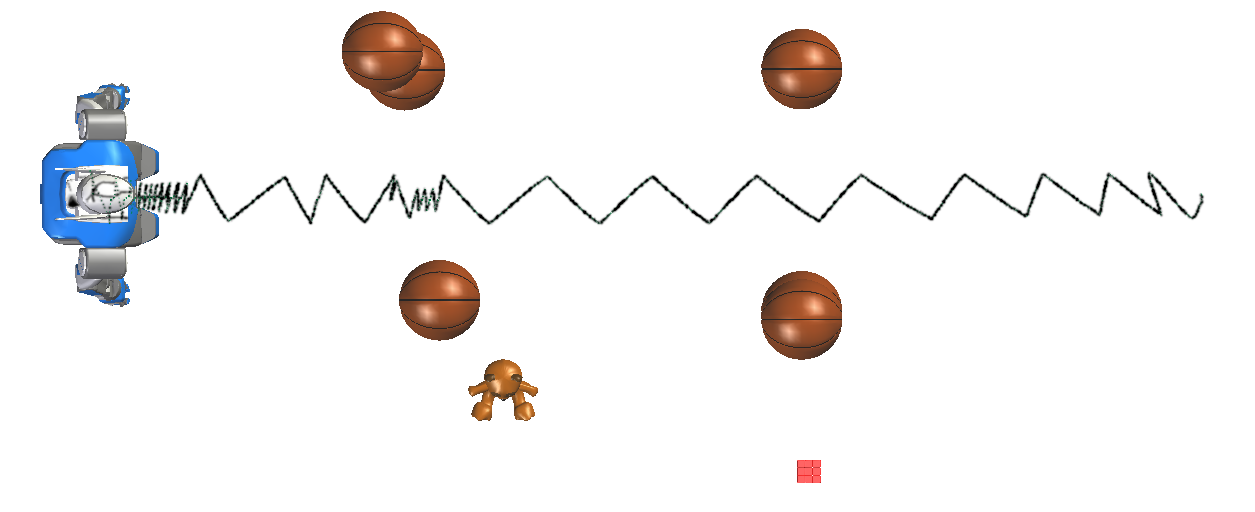
\includegraphics[width=0.7\linewidth]{pics/objects-cloud/waist-trajectory.png}

  \caption{Horizontal trajectory of the robot waist during
    locomotion.}
  \label{fig:cluttered-waist} 
\end{figure}


\subsection{Grasp Planning}

The problem shown in Fig. \ref{fig:grasp} is defined as a grasping task. 
The final configuration is defined implicitly by a desired hand
position. We generated automatically goal configurations solving the
task by following the method proposed in \cite{dalibard09}. Then, we applied our
planner to generate a whole-body walk motion that solved the grasping
task. Computation time for the first planning phase was on average
83.0~s, and the animation of the trajectory presented on
Fig. \ref{fig:grasp} used 90.1~s.  
Fig. \ref{fig:grasping-waist} 
shows the robot waist trajectory during locomotion.



\begin{figure}[h!]
\centering
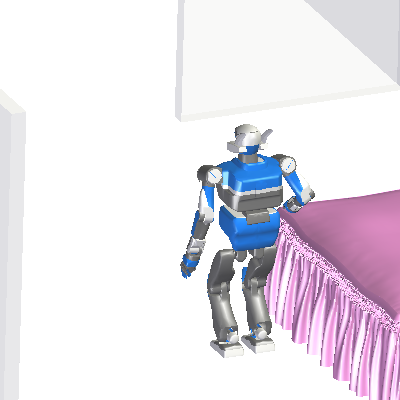
\includegraphics[width=0.24\linewidth]{pics/apartment/trajectory-1.png}
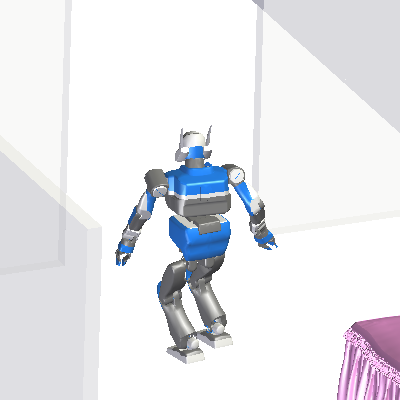
\includegraphics[width=0.24\linewidth]{pics/apartment/trajectory-2.png}
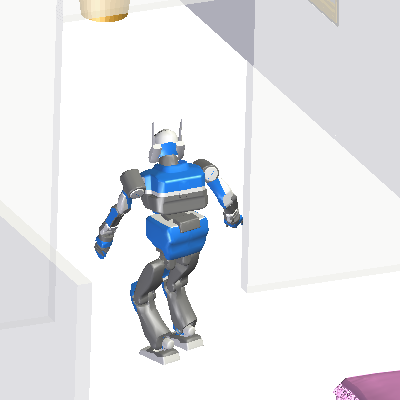
\includegraphics[width=0.24\linewidth]{pics/apartment/trajectory-3.png}
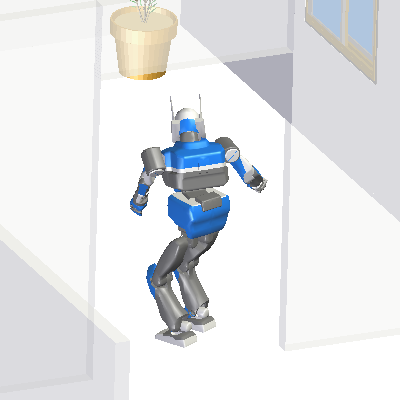
\includegraphics[width=0.24\linewidth]{pics/apartment/trajectory-4.png}
\\ 
\vskip 0.1cm
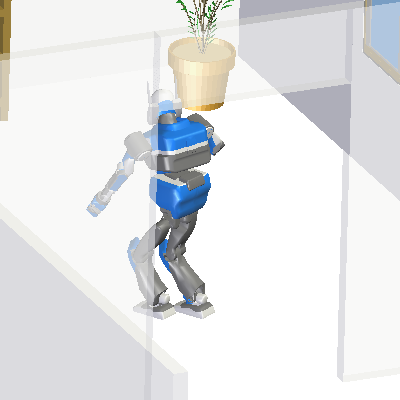
\includegraphics[width=0.24\linewidth]{pics/apartment/trajectory-5.png}
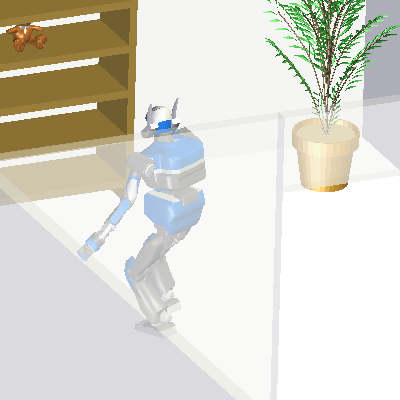
\includegraphics[width=0.24\linewidth]{pics/apartment/trajectory-6.png}
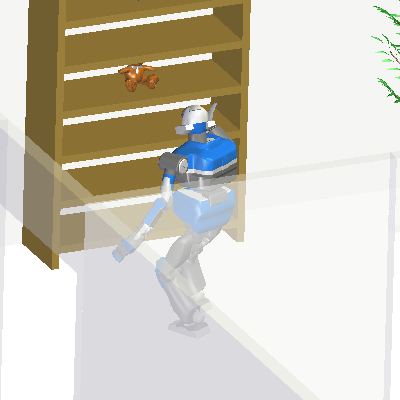
\includegraphics[width=0.24\linewidth]{pics/apartment/trajectory-7.png}
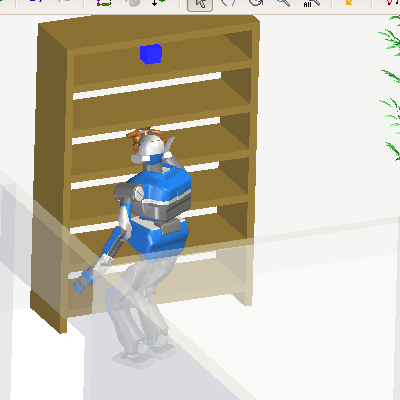
\includegraphics[width=0.24\linewidth]{pics/apartment/trajectory-8.png}

\caption{Solution path for a grasp planning problem in an
  appartment. The goal is implicitly defined as an inverse kinematics
  task.} 
\label{fig:grasp}
\end{figure}




\begin{figure}[h!]
\centering

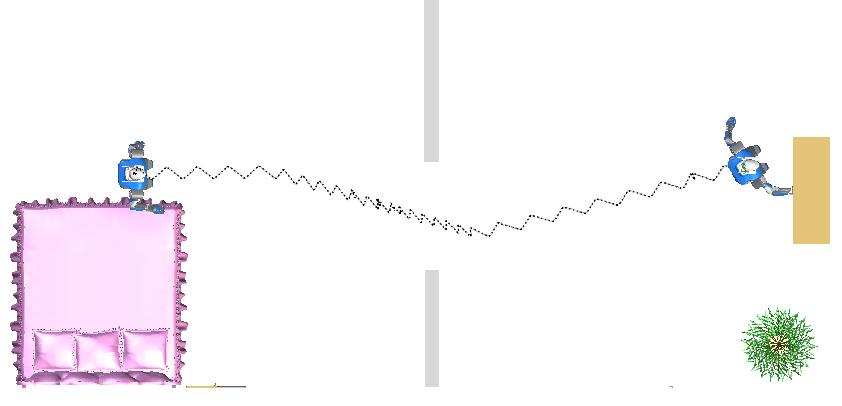
\includegraphics[width=0.9\linewidth]{pics/apartment/waist-trajectory.png}


\caption{Horizontal trajectory of the robot waist during
    locomotion.}
\label{fig:grasping-waist}
\end{figure}


\section{Conclusion and perspectives}

In this paper, we have presented a new planning strategy for humanoid whole-body
motion planning including locomotion. The algorithm is based on a formal
small-space controllability property of humanoid robots. 
We have used our motion planner on different examples, and validated the
generated motions on a real robot.
Our method has some limitations that should be addressed in future work:
\begin{itemize}
\item Because of the kinematic constraints we apply at the planning stage, we are not
	able yet to plan motions where the robot steps over obstacles, while this is an 
	important feature of humanoid robots.
\item The fact that we use the simplified cart-table model forces us to keep the CoM
	of the robot at a constant height. A more complete model could allow us to plan
	other types of locomotions, for example to allow the robot to pass under 
	obstacles. We will try to integrate the possibilities 
        presented in \cite{kanehiro2004locomotion} and prove the small-space controllability
        result for a more general walking humanoid robot model.
\end{itemize}

\section{Acknowledgments}

This work was supported by the French FUI Project ROMEO and the European Project ECHORD-231143. 
The authors would like to thank warmly Thomas Moulard and Olivier Stasse for their valuable help during experiments.

\section*{Appendix: Trajectory following with small CoM Motions}


The  CoM  and ZMP  motions  presented in Sec. \ref{sec:com-stc} 
 can  be  adapted to  walk
in-place  at  a position  $(x_0,y_0,\theta_0)$. The coordinates  of the
left foot center are given by: 
$foot_l(x_0,y_0,\theta_0) = (\left( x_0 - L  \sin (\theta_0), y_0 + L \cos
(\theta_0)\right)$
and of the right foot center: 
$foot_r(x_0,y_0,\theta_0) = \left( x_0 + L  \sin (\theta_0), y_0 - L \cos
(\theta_0)\right)$. Let us  note $c_0(x_0,y_0,\theta_0) : \mathbb{R}_+
\rightarrow \mathbb{R}^2$ the corresponding CoM motion:

\[
c_0(x_0,y_0,\theta_0)(t) = 
\left(
\begin{array}{c}
x_0 - \epsilon \sin (\theta_0) \sin (\omega t) \\
y_0 + \epsilon \cos (\theta_0) \sin (\omega t) 
\end{array}
\right)
\]
This motion stays in a  ball of size $\epsilon$ around $(x_0,y_0)$ and
generates a  ZMP motion that  reaches successively the centers  of the
feet. Let us note it $zmp_0(x_0,y_0,\theta_0)$:
\[
zmp_0(x_0,y_0,\theta_0)(t) = 
\left(
\begin{array}{c}
x_0 - \epsilon (1+\left( \frac{\omega}{\omega_0} \right)^2)\sin ( \theta_0) \sin (\omega t)   \\
y_0 + \epsilon (1+\left( \frac{\omega}{\omega_0} \right)^2)\cos ( \theta_0) \sin (\omega t)
\end{array}
\right)
\]

Let us now describe the CoM and legs motions starting from a static configuration $q_i$ 
and reaching a configuration $q_f = (x_f,y_f,\theta_f)$. Without loss of generality, one can
assume that $q_i = (0,0,0)$. We consider as given the transient state that initializes a walk
in-place motion. At time $(t=0)$, the robot is walking in-place and the CoM and ZMP are 
moving towards the left foot.

Let $f : [0,T] \rightarrow [0,1]$ be an increasing function of class $C^\infty$  such  
that  $f(0)  =  0$, $\dot{f}(0) = 0$, $\ddot{f}(0) = 0$, $f(T) = 1$, $\dot{f}(T) = 0$ and
$\ddot{f}(T) = 0$. One can write explicitly such a function by using a degree 5 spline.
In order to bound the variations of the ZMP trajectory due to variations of $f$, we also 
request the successive derivatives of $f$ to be bounded, and require
that for all $t \in [0,T]$:
\[
\begin{array}{rcl}
\frac{1}{\omega_0^2}(|x_f|+|y_f|)|\ddot{f}(t)| & < &
\min(l_1/6,l_2/4)\\
\frac{2\epsilon\omega}{\omega_0^2}|\theta_f||\dot{f}(t)| & < & l_1/6
\\
\frac{\epsilon}{\omega_0^2}|\theta_f||\ddot{f}(t)| & < & l_1/6 \\
\frac{\epsilon}{\omega_0^2}\theta_f^2\left(\dot{f}(t)\right)^2 & < &
l_2/4
\end{array}
\]


Again, these inequalities can be guaranteed by choosing $T$ large
enough, i.e. by following the path slowly enough. The $\mathcal{CS}$
trajectory $f_{\mathcal{CS}} : [0,T] \rightarrow \mathcal{CS}$ such
that for all $t \in [0,T],f_{\mathcal{CS}}(t) = f(t)(q_f - q_i)$ goes
from $q_i$ to $q_f$ in time $T$, while staying on the segment
$[q_i,q_f]$. The CoM motion designed to follow this trajectory by
walking is:
\[
\label{eq:com-walk}
c(t) = c_0 (f_{\mathcal{CS}}(t)) =
\left(
\begin{array}{c}
f(t) x_f - \epsilon \sin ( f(t) \theta_f) \sin (\omega t) \\
f(t) y_f + \epsilon \cos ( f(t) \theta_f) \sin (\omega t)
\end{array}
\right)
\]

Note that the initial conditions on $f$ guarantee the continuity of
the command derivative and of the ZMP position at time $(t=0)$. The
desired ZMP trajectory is:

\[
zmp_{ref}(t) = 
\left(
\begin{array}{c}
f(t) x_f - \epsilon (1+\left( \frac{\omega}{\omega_0} \right)^2)\sin ( f(t) \theta_f) \sin (\omega t)   \\
f(t) y_f + \epsilon (1+\left( \frac{\omega}{\omega_0} \right)^2)\cos ( f(t) \theta_f) \sin (\omega t)
\end{array}
\right)
\]

Following this trajectory, at time $t_l^{(n)}$, the ZMP is located at the center of the left foot,
the robot can lift its right foot and move it to position $foot_r(c(t_r^{(n)}))$ and at time 
$t_r^{(n)}$, the ZMP is located at the center of the right foot, the robot can lift its left foot
and move it to position $foot_l(c(t_l^{(n+1)}))$. The real ZMP trajectory $zmp_{real}$ 
differs from  $zmp_{ref}$ because of variations of $f$. One can compute $zmp_{real}$
by calculating the successive derivatives of $c$. The error between the desired ZMP position
and its real position at time $t$ is given by the equation:
\[
  \begin{array}{cl}
    zmp_{ref}(t) - zmp_{real} = &
    -\frac{1}{\omega_0^2} \ddot{f}(t)
    \left(
    \begin{array}{c}
      x_f \\
      y_f
    \end{array}
    \right) \\
    &
    +
    \frac{2\epsilon \omega}{\omega_0^2} \theta_f \dot{f} (t) \cos(\omega t)
    \left(
    \begin{array}{c}
      \cos( f(t) \theta_f) \\
      \sin( f(t) \theta_f)
    \end{array}
    \right) \\
    &
    +
    \frac{\epsilon}{\omega_0^2} \theta_f \ddot{f} (t) \sin(\omega t)
    \left(
    \begin{array}{c}
      \cos( f(t) \theta_f) \\
      \sin( f(t) \theta_f)
    \end{array}
    \right) \\
    &
    -
    \frac{\epsilon}{\omega_0^2} \theta_f^2 \dot{f} (t)^2 \sin(\omega t)
    \left(
    \begin{array}{c}
      \sin( f(t) \theta_f) \\
      \cos( f(t) \theta_f)
    \end{array}
    \right)
  \end{array}
\]

At time $t$, the vector 
$\left(
\cos( f(t) \theta_f) ,
\sin( f(t) \theta_f)
\right)$ 
follows the robot orientation.
Using the bounds on the derivatives of $f$, one can check that 
the ZMP error along this vector is less than 
$l_1/2$. In the same way, the error along the direction orthogonal to the robot
is less than $l_2/2$. Therefore, for all $n$, at time $t^{(n)}_l$, the ZMP is under the left
foot and at time $t^{(n)}_r$ the ZMP is under the right foot. During the double support
phases, the ZMP also stays inside the support polygon.

Overall, we have found a stable walk motion that goes from $q_i$ to $q_f$ while
keeping the CoM within $\epsilon$ distance of the line segment between $q_i$ 
and $q_f$. Once in $q_f$, a $C^1$ command can switch 
to a walk in-place trajectory then to a static configuration.



\bibliographystyle{agsm}   


\bibliography{bibli}






\end{document}


